\chapter{Introduction}
\label{introduction}

\begin{description}
\item[Problem definition]: Reverse engineering binary programs can help to find vulnerabilities in software, this is a hard task that depends on the skill of the reverse engineer. Decompilers exist to help in this process, but their output is still difficult to read and understand.

\item[Significance]: Making reverse engineering easier can help to find vulnerabilities, help researchers quickly understand novel malware, replicate software of which the source code is lost, discover illegitimate usages of intellectual property, porting abandonware, etc.

\item We therefore propose our code summarization solution, which takes decompiled functions and synthesizes summaries.

\item Our main contributions are a pre-trained fine-tuned code-summarization model, to create this model we explored the influence of the input types, the impact of data duplication, the impact of different aspects of stripped code and pre-training on the model performance. We also provide a novel dataset with aligned source-code, decompiled code and comments, for both stripped and unstripped code.
\end{description}
\newpage

\section{Problem Definition}
%Rewrite this
Reverse Engineering (RE) the inner workings of binary executables is required analyse and understand programs. Furthermore, it can be used to find vulnerabilities and to analyse novel malware. Unlike binaries, the source code is relatively easy to read. The source code of the binaries is, however, not always available. The original code gets compiled into a runnable binary program by compilers such as Clang/LLVM \footnote{Clang: https://clang.llvm.org/} or GCC \footnote{GCC: https://gcc.gnu.org/} and delivered to the user.

To understand what a binary program does exactly, the binary code can be decompiled into readable code by decompilers such as Ghidra\footnote{Ghidra Framework: url{https://ghidra-sre.org/}} and IDA Pro\footnote{IDA Pro: url{https://hex-rays.com/ida-pro/}}. Understanding decompiled code is still intrinsically difficult process. It is a manual, time-consuming process and still largely depends on the skill of the Reverse Engineer\cite{TypeInferenceSurvey}.

A large part of the work that goes into reverse engineering a binary is spent labeling functions with semantic information \cite{reverseEngineerProcess}. In the source code domain, automatic code-summarization is \cite{recommend_summarization} used to automatically generate short natural language descriptions of source code. The summaries generated by these models are supposed to mimic the single sentence comments or descriptions that are included in source code. While these methods have been successfully applied syntactically-rich to programming languages such as Python, Java and PHP\cite{CodeT5, CodeBERT, CodeX}, none of these methods have been applied to the relatively syntactically-poor output of decompilers.

\section{Relevance}
Besides from analysing malware and finding vulnerabilities, reverse engineering can be used to find vulnerabilities, help researchers quickly understand novel malware, it can help with fingerprinting existing malware \cite{TypeInferenceSurvey}, replicate software of which the source code is lost, discover illegitimate usages of intellectual property, porting abandonware, and more\cite{TypeInferenceSurvey}. Furthermore, the binaries are the most accurate representation of the program that actually runs on the system, there is no guarantee that the source code actually represents the binary that is delivered to the user \cite{TypeInferenceSurvey}. 
\subsection{Stakeholders}
There are several stakeholders who might benefit from this research. Firstly, security researchers who aim to understand malware. This could help them understand and reverse engineer novel malware more quickly. 

Users of closed-source software can use this to inspect the software for faults. Closed source software can be patched, rewritten and reused to serve their exact purposes. Furthermore, an understanding of the source code can allow users to change the binary in memory during runtime. A malicious example of this group is game hackers who change certain memory addresses to give themselves an unfair advantage (changing their health points for instance) \cite{TypeInferenceSurvey}. 
Reverse engineers who aim to replicate closed-source software or software of which the source code is lost. This research can be used to help create open-source copies or to port the software to newer architectures. Examples range from porting old abandoned open-source projects, to porting abandonware (on which copyrights still apply), or even the theft of intellectual property from closed source commercial software.

On the flip side, creators of closed source software can use reverse engineering to determine whether other software has copied their products and infringed on their intellectual property.

Lastly, developers of reverse engineering programs and tool-kits might be able to use the results of this research to enhance their own products. 

\section{Contributions}
We therefore propose our code summarization model, which takes decompiled functions and synthesizes summaries \ref{img:usecase}. The starting point for a reverse engineer is a binary that has been compiled by a compiler from source code. This binary can then be fed into a reverse engineering tool like Ghidra, which will decompile the binary. From this decompiled code the functions can then be extracted, this is a relatively simple process. These decompiled functions can then be summarized using our trained model.

\begin{figure}[htb]
    \centering
    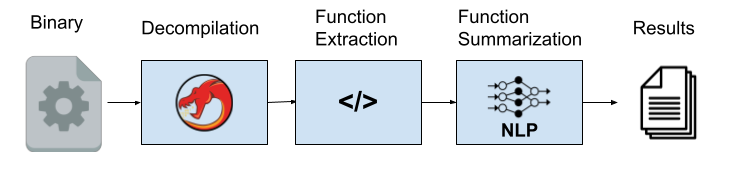
\includegraphics[width=\textwidth,height=\textheight,keepaspectratio]{img/UseCase.png}
    \caption{Proposed solution}
    \label{img:useCase}
\end{figure}

Our main contributions can be summarized as follows:
\begin{description}
 \item[Model:] Our main contribution is a pre-trained fine-tuned code-summarization model for decompiled and stripped-decompiled code. The model uses CodeT5 and is fine-tuned and evaluated on our own dataset of source code, decompiled code and stripped-decompiled code pairs. 
 \item[Impact study:] To create this model we explored the influence of the input types, the impact of data duplication, the impact of different aspects of stripped code on the model performance.
 \item[Pre-training:] To improve the performance of the model we implemented and evaluated the Masked Language Modeling (MLM), translation, deobfuscation (DOBF) and span-detection (SPAN) pre-training objectives. 
 \item[Dataset:] Finally we contribute the dataset used to fine-tune and pre-train the model. The dataset contains aligned comment-source code, comment-decompiled code, comment-stripped-decompiled code pairs. We also provide a synthetic dataset of comment-demi-stripped code pairs. Furthermore, we provide the data used by the pre-training objectives. This is a novel dataset which can be used by other works to train and evaluate their models.
\end{description}

\section{Structure}
The rest of the thesis is outlined as follows: Chapter \ref{background} will consist of a brief introduction and explanation of concepts and tools used throughout the thesis. In chapter \ref{relatedWork} we will discuss other relevant works in this field.  Chapter \ref{methodology}  will cover the research methodology, the experimental setup will be covered in chapter \ref{ExperimentalSetup}. The results will be presented in chapter \ref{results}, followed by a discussion on the findings in chapter \ref{discussion}. Finally, chapter \ref{conclusion} will summarize and conclude on the findings, discuss possible future works and feature a short discussion on the threats to validity.